\documentclass{ximera}

\input{../../preamble.tex}

\author{Elizabeth Campolongo}
%\acknowledgement{https://www.stitz-zeager.com/szca07042013.pdf}

\begin{document}
\begin{exercise}

It's a beautiful day and you decide to go to the park and fly a kite. The wind is stronger than expected and the string has completely unspooled, that's 500ft! Could this be a new kite-flying record? The angle the string is making off the spool (if you place it on the ground) is 85$^\circ$.


\begin{enumerate}

\item We begin with a picture of the problem. 

		\begin{image}[2in]
		  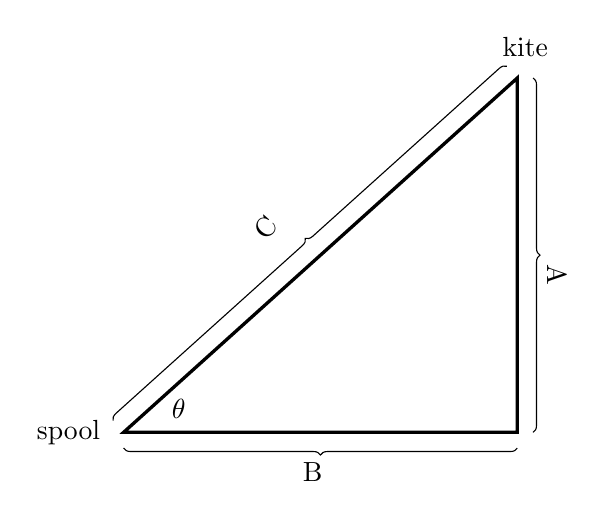
\begin{tikzpicture}
		    \coordinate (C) at (-1,2);
		    \coordinate (D) at (4,2);
		    \coordinate (E) at (4,6.5);
		    \tkzMarkRightAngle(C,D,E)
		    \tkzMarkAngle(D,C,E)
		    \draw[decoration={brace,mirror,raise=.2cm},decorate,thin] (-1,2)--(4,2);
		    \draw[decoration={brace,mirror,raise=.2cm},decorate,thin] (4,2)--(4,6.5);
		    \draw[decoration={brace,raise=.2cm},decorate,thin] (-1,2)--(4,6.5);
		    \draw[very thick] (D)--(E)--(C)--cycle;
		    \node at (1.4,2-.5) {B};
		    \node[rotate=-90] at (4+.5,4) {A};
		    \node[rotate=48.5] at (.8,3.8+.8) {C};
		    \node at (-.3,2.3) {$\theta$};
		    \node at (-1.7,2) {spool};
		    \node at (4.1,6.9) {kite};
		  \end{tikzpicture}
		\end{image}

Label all known lengths with units.
\begin{enumerate}
\item Side $A$ is the $\wordChoice{\choice[correct]{height}\choice{distance}}$ of the kite and what we want to find.

\item Side $B$ is the $\wordChoice{\choice{height}\choice[correct]{distance}}$ to the kite along the ground.

\item Side $C$ is the length of the string and it is $\answer{500}$ft long.

\item $\theta$ = $\answer{\frac{5\pi}{12}}$ radians

\end{enumerate}

\item \begin{exercise}
Now that we have a labeled picture, let's find the height of the kite. Give exact values.
\begin{enumerate}
\item The height of the kite is $A = \answer{125(\sqrt{6}+\sqrt{2})}$ ft.

\item The distance to the kite is $B = \answer{125(\sqrt{6}-\sqrt{2})}$ ft.

\item The angle between the kite and a vertical line from the kite to the ground is $\answer{\frac{\pi}{12}}$ radians.
 
 \end{enumerate}	
 
For fun, the actual highest a kite has been flown was 16,009 ft (4,879.54m) by Robert Moore in 2014 in Australia. (Courtesy of Guinness World Records)
\end{exercise}
\end{enumerate}

\end{exercise}
\end{document}